% ═══════════════════════════════════════════════════════════════════════
\section{Un peu d'histoire}
% ═══════════════════════════════════════════════════════════════════════

\begin{frame}{Note historique 5.1 --- Karl Pearson (1857--1936)}
  \footnotesize
  \begin{columns}[T]
    \begin{column}{0.25\textwidth}
      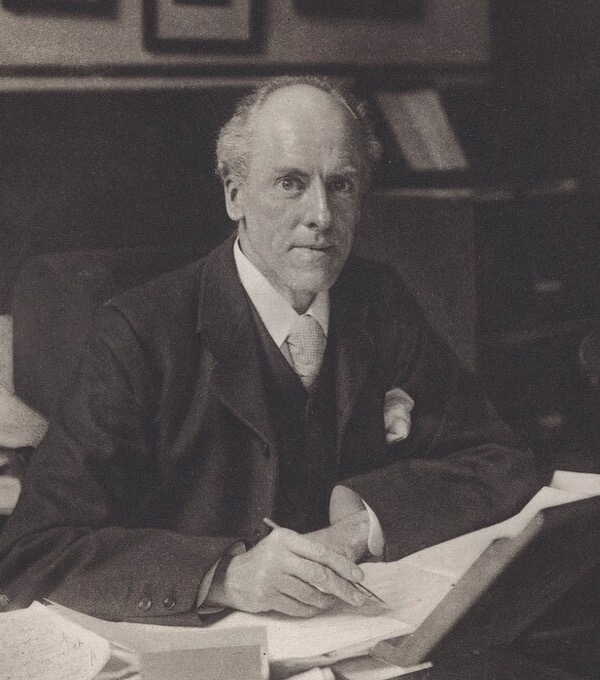
\includegraphics[width=\linewidth]{karl-pearson.jpg}\\
      {\scriptsize\color{gray}En 1910. Domaine public, National Portrait
      Gallery (Londres), Wikimedia Commons.}
    \end{column}
    \begin{column}{0.72\textwidth}
      \begin{itemize}
        \item Né à Londres ; mathématiques à Cambridge, puis physique,
          philosophie et droit en Allemagne. En 1884, professeur de
          mathématiques appliquées à l'University College de Londres.
        \item Sous l'influence de Galton et de Weldon, il se tourne vers
          l'étude statistique de l'hérédité et de l'évolution : la
          biométrie.
        \item L'un des fondateurs de la statistique moderne : l'expression
          « écart type », le coefficient de corrélation, le test du
          khi-deux, la revue Biometrika (1901).
        \item 1901 : « Sur les lignes et les plans qui s'ajustent au plus près
          à des systèmes de points de l'espace ».
      \end{itemize}
    \end{column}
  \end{columns}
\end{frame}

\begin{frame}{Note historique 5.1 (suite)}
  \small
  \begin{itemize}
    \item Pearson remarque que les deux droites de régression dépendent de
      la variable que l'on choisit d'expliquer.
    \item Il propose de minimiser la somme des carrés des distances
      perpendiculaires : exactement le problème de la section 2.
    \item Il montre que cette droite passe par le centre de gravité et
      qu'elle est portée par le grand axe de l'« ellipsoïde de corrélation »
      --- un vecteur propre de la matrice de covariance.
    \item Comme Galton, il fut un ardent défenseur de l'eugénisme ; en 1911,
      premier titulaire de la chaire d'eugénisme créée par le testament de
      Galton. Ces idées, qui ont servi à justifier des stérilisations
      forcées au \siecle{20}, sont aujourd'hui unanimement rejetées ; en
      2020, l'University College a retiré leurs noms de plusieurs
      bâtiments.
    \item Des outils mathématiques solides peuvent être mis au service de
      projets condamnables.
  \end{itemize}
\end{frame}

\begin{frame}{Hotelling, Spearman et la suite}
  \small
  \begin{itemize}
    \item Harold Hotelling (1895--1973) redécouvre la méthode et lui donne
      son nom (1933) : « Analyse d'un ensemble de variables statistiques en
      composantes principales », dans le Journal of Educational Psychology,
      sur des résultats d'élèves en lecture et en arithmétique.
    \item Le contexte : Spearman (1904) avait observé que les notes
      d'écoliers dans toutes les matières sont corrélées positivement, et en
      avait déduit un facteur général d'intelligence, $g$. Nos six élèves,
      dont l'axe principal mesure le « niveau général », en sont un écho
      lointain.
    \item Hotelling propose une méthode itérative de calcul, voisine de la
      méthode des puissances du chapitre 4.
    \item Longtemps limitée par le calcul (une matrice $10\times10$ à la
      main : plusieurs jours de travail), l'ACP se répand avec les
      ordinateurs. En France, l'école d'« analyse des données » de
      Jean-Paul Benzécri (années 1960--1970).
    \item Autres noms : la transformation de Karhunen--Loève en traitement du
      signal. Aujourd'hui, l'une des méthodes les plus employées de la
      statistique.
  \end{itemize}
\end{frame}
